 % \chapter{Introduction}
\chapter[Salt Rejection Through Gated Nanoporous Graphene]{Understanding Macroscopic Salt Rejection Through Gated
  Nanoporous Graphene}
\label{ch:np}
\renewcommand*\imgdir{img/ch-np/}
% \newcommand*\Fig{Figure}

% \dictum[Wolfgang Pauli]{%
  % God made the bulk;\\Surfaces were invented by the devil
  % }%
\worktodo{find the quote or quit}

\vspace{1em}

\chapterabstract{Part of this chapter appears in the following journal
  article: Wyss, R. M., Tian, T., Yazda, K., Park, H. G. \& Shih,
  C.-J. Macroscopic Salt Rejection through Electrostatically Gated
  Nanoporous Graphene. Nano Lett. 19, 6400–6409 (2019).
 }

\section{Introduction}
\label{sec:intro}

%
A central objective in nano\-science is to control
transport phenomena at nanometer scale to explore new technological
opportunities.  The reduction of characteristic dimensions gives rise to substantially different transport
properties in comparison to their bulk counterparts
\cite{Schoch_2008_nanofluid}.
%
One well-known example is the nanopores, in which the effect of
surface-mediated transport becomes dominant when the pore size is
comparable to the characteristic length of diffusion, enabling new
applications such as ionic diodes
\cite{Karnik_2007_nanofluidic,Siwy_2002_fabrication_NPore,Vlassiouk_2007_nanofluidic},
field-effect transistors \cite{Nam_2009_IFET_sub10nm}, desalination
\cite{Heiranian_2015_desali}, and nanopore-based DNA sequencing
\cite{Heerema_2016_gr_np_DNA,Garaj_2013_hugging_gr_pore}.
%
In this sense, atomically thin 2D material are not only attractive due
to their unique electronic properties, but also as the thinnest
membrane materials allowing ultimate permeation when combining with
nanopores
~\cite{Suk_2010_water_PG,Jiang_2009_PG_gas,Celebi_2014_science,Koenig_2012,Drahushuk_2012_gas_permeation_gr}.
%
Early research has shown the potential of desalination using graphene
with sub-nanometer pores, which hinders ion passage without losing
water permeability
\cite{Cohen_Tanugi_2012,Suk_2014_ion_sub_5nm,Cohen_Tanugi_2014_permeab,Cohen_Tanugi_2015_PG,O_Hern_2014_ion,O_Hern_2015_ion_gr,Surwade_2015_desali_npg,Walker_2017_cation_select_2D,Ghosh_2018_PG_ion}.
Nevertheless, there are still several technical issues to be solved.
In practice, the fabrication of sub\-nanometer pores in
a 2D material sheet with atomic precision and over a large area with
atomic precision, still remains challenging.
\cite{Suk_2014_ion_sub_5nm,Rollings_2016_gating,O_Hern_2012_defect,Wang_2017_mechanism_thin_membrane}.
%
Moreover, a small portion of excessively large pores or defects can
significantly deteriorate the membrane performance.
%
% Regarding these
% issues, we have previously developed a highly-scalable technique to
% fabricate uniformly-distributed nanopores (sub-20 to 50 nm) over
% wafer-scale graphene samples \cite{Choi_2018_wafer_scale_gr}.
A major step towards the real-world desalination and separation
applications of nanoporous 2D material membranes, would be to develop
methodology that allow appreciable selectivity while the pore size can
be even larger than the hydration radii.
% Therefore, it is critical to develop methodology that
% allow appreciable selectivity of nanoporous 2D membrane even with
% large pore size.

Inspired by the ion channels in cellular membranes\worktodo{cite}, the
selectivity of nanopores can not only be controlled by size-exclusion,
but also by engineering the surface charge and potential.
%
A number of recent reports have explored the effect of surface charges
on the selectivity of ion transport through graphene nanopores, as a
consequence of the electrostatic interactions between solvated ions
and the charged functional groups attached on graphene, indicating
that ion selectivity can exists in pores with diameter even as large
as 30 nm~\cite{Rollings_2016_gating,Surwade_2014_carbon_electrochemical_ion}.
%
However, it remains controversial if the surface charges can result in
a degree of salt rejection, as the surface charge / potential in these systems
cannot be precisely quantified, which are sensitive to the surroundings
as well as the history of chemical treatment
\cite{Li_2008_gr_suspension}.
%
A fundamental understanding of the interactions between the charged 2D
nanopores and the electrolyte solution, especially the mechanism of
ion transport through these nanopores, is still absent.

In this chapter, combining experimental and theoretical studies, we
investigate electrolyte permeation through centimeter scale,
electrostatically gated nanoporous graphene membranes, with pores that
are in the order of $\sim{}$\unit[20]{nm}.
%
We find that electrostatic gating can effectively reduce ion transport
through these membranes, despite the pore size is significantly larger
than the hydration radii of the ions. We model the surface potential
around the graphene nanopores, by taking into account the elementary
electronic properties of graphene (\eg the quantum capacitance).
%
The interplay between graphene quantum capacitance and the electrical
double layer is found to selectively modulate the anionic and cationic
transport paths, creating voltage-dependent electrochemical barriers
when the pore size is comparable to the Debye screening length. Our findings
reveal a new degree of freedom regulating electrolyte permeation
through porous two-dimensional materials, complementary to the pore
size design and engineering.

\section{Results and discussions}
\label{sec:np-res}

\subsection{Experimental Observations}
\label{sec:np-exper-observ}

The experimental realization of electrostatically-gated nanoporous
graphene membranes are carried out in the group of Prof. H. G. Park
\worktodo{check} in ETH Zürich. 
%
 \autoref{fig:np-1}a depicts the experimental setup characterizing
ionic diffusion through a sheet of double layer porous graphene
(PG).
%
Two reservoirs, namely the high-concentration reservoir (HCR)
containing electrolyte solution with molar concentration $c_0$, and
the low-concentration reservoir (LCR) containing de-ionized (DI)
water, are separated by a PG membrane supported by a polycarbonate
track-etched (PCTE) film.
%
Magnetic stirrers are used to minimize the effects of external
concentration polarization in both reservoirs.
%
A conductivity
probe is placed in the LCR to monitor the ionic concentration as a
function of time. The membrane is attached to a piece of copper tape
connected to a voltage source applying an electrical bias
$V_{\mathrm{G}}$, with the LCR grounded ( \autoref{fig:np-1}a
inset).
%
The structure of the PCTE-supported PG membrane is schematically shown in
\autoref{fig:np-1}b, using the protocol developed in 
\cite{Choi_2018_wafer_scale_gr}. 
which enables formation of
%20191017--here
uniformly-distributed graphene nanopores over large area up to 25
cm$^{2}$ (details see Supplementary Section \autoref{SI-sec:exp}). The
normally distributed, circular pores with pore diameters of 20$\pm$10
nm and a pore density of 1.25$\pm$0.25$\times$10$^{10}$ cm$^{-2}$ (
\autoref{fig:np-1}c inset) over a large area were perforated on
graphene.  By optimizing the subsequent transfer process, a high
surface coverage ($>$ 98\%) of PG on PCTE was obtained (
\autoref{fig:np-1}c), allowing reliable characterization of the ion
transport behavior (details see Supplementary Section
\autoref{SI-sec:exp}).  The system presented here allows us to
systematically investigate the diffusive flux of ions across a sheet
of PG, $\boldsymbol{J}$, driven by the gradient of electrochemical
potential in the electrolyte medium.

First, the control experiments were carried out by measuring the ionic
diffusion of seven salt species, including KCl, NaCl, LiCl,
K$_{2}$SO$_{4}$, MgSO$_{4}$, CaCl$_{2}$ and K$_{3}$[Fe(CN)$_{6}$],
through the bare PCTE membrane at $c_{0}$ = 0.1 mM. As the diffusive
flux is comparably small, the conductivity increases linearly with
time in the LCR (e.g.  \autoref{fig:np-2}a) within the measurement
duration (1 h), suggesting the concentration gradient across the
membrane remains constant. The diffusive fluxes (blue bars in 
\autoref{fig:np-2}b) of different salts were obtained by converting the
conductivity-time profiles using calibration curves (Supplementary
Section \autoref{SI-sec:measure}). The theoretical diffusive fluxes
through PCTE are obtained based on the assumption that the membrane
consists of cylindrical pores with uniform diameter and a low
tortuosity $\tau$ of $\sim{}$1.2 \cite{O_Hern_2012_defect}:
\begin{equation}
  \label{eq:np-j-pcte}
  \boldsymbol{J}_{\mathrm{PCTE}} = \frac{\pi r_{\mathrm{PCTE}}^{2} N_{\mathrm{p}} D_{\mathrm{\pm}} \Delta c}{L \tau}
\end{equation}
{where $r_{\mathrm{PCTE}}$ (= \unit[200]{nm}) is the PCTE pore radius, $N_{\mathrm{p}}$  (= \unit[$1.5\cdot10^{12}$]{m$^{-2}$}) is
numbers of pore per area, $D_{\mathrm{\pm}}$ is the salt diffusivity
(average of cation and anion diffusivity), $\Delta c$ is the bulk
concentration difference between two reservoirs, i.e.,
$\Delta c \sim c_{0}$ and $L$ (= \unit[24]{$\mu$m}) is the thickness of the PCTE membrane.
By using the salt diffusivity values (Supplementary Table
\autoref{SI-tab:diff}), the calculated diffusive fluxes (red bars in
 \autoref{fig:np-2}b) show reasonable agreement with the experimental
values.}

Next, we carried out the same experiments using the PG-covered PCTE
membrane (PG-PCTE), without electrostatic gating. The measured
diffusive flux values, $\boldsymbol{J}_{\mathrm{PG0}}$ (green bars in
 \autoref{fig:np-2}b), remain at the same order of magnitude compared
with those of bare PCTE membrane, suggesting that the transport
resistance of PCTE $R_{\mathrm{PCTE}}$, is dominant over that of PG
without gating, $R_{\mathrm{G}}^{0}$. Using a simple circuit model, we
estimate the ratio $\delta$ between $R_{\mathrm{G}}^{0}$ and
$R_{\mathrm{PCTE}}$, i.e.,
$\delta = R_{\mathrm{PCTE}}/R_{\mathrm{G}}^{0}$, to be $\sim$2.2,
which is in good agreement with the value derived from the
experimental data in  \autoref{fig:np-2}b (details see Supplementary
Section \autoref{SI-sec:R-model}).
% \todo[inline]{Make sure that the
  % values used are correct.}


\subsection{Salt rejection induced by electrostatic gating}
\label{sec:res-2}

We next discuss the effects of electrostatic gating on graphene. 
{ Electrostatic gating has been employed previously to alter the 
ion permeation through nanoporous structures. For example, an applied bias on a mesoporous 
carbon membrane, having pores of $<$\unit[5]{nm}, allows to stop the 
ion flux once the Debye length of the solution approaches the pore size \cite{Surwade_2014_carbon_electrochemical_ion}. 
Similar experiments using nanoporous gold membranes, however, find that the cation and anion 
transport is enhanced upon applying a bias \cite{Mccurry_2017_electrolyte_porus_gold}. While the former behavior 
was ascribed to the depletion of the channel from ions upon gating, the latter was a result of enhanced transport
by dominating drift currents.}


In order to investigate the behavior in more detail, the ``three-interval'' method, which has been used
in controlling the membrane potential in mesoporous carbon membranes
\cite{Surwade_2014_carbon_electrochemical_ion}, is adopted here.  \autoref{fig:np-2}a
illustratively represents how the measured conductivity evolves with
time. Specifically, in the first interval, the gate voltage source is
turned off and the conductivity probe is on, allowing us to obtain the
conductivity-time profile with an average slope $s_{1}$ that
corresponds to the diffusive flux across the PG-PCTE membrane. In the
second interval, a voltage $V_{\mathrm{G}}$ is applied to the membrane
after turning off the conductivity probe, followed by the third
interval $s_{3}$, in which the conductivity probe is turned on again
to give the corresponding slope. A control experiment was performed to
ensure the copper tape was not in direct contact with the ionic
solution (Supplementary Section \autoref{SI-sec:copper}). The slope
corresponding to the second interval $s_{2}$, as the conductivity
probe is off, is determined by linear interpolation of the
conductivities from the endpoint of interval 1 to the starting point
of interval 3. A decrease of slope observed in interval 2 indicates
that the total flux through PG-PCTE is reduced upon gating (i.e. salt
penetration through the PG pores is hindered). We define such
experimentally measured reduction rate as $\eta$, which is equivalent
to the decrease of total diffusive flux through PG-PCTE as follows:
\begin{equation}
  \label{eq:np-rejection}
  \eta = \frac{\bar{s} - s_{2}}{\bar{s}} = \frac{\boldsymbol{J}_{\mathrm{PG0}}
    - \boldsymbol{J}_{\mathrm{PG}}(V_{\mathrm{G}})}{\boldsymbol{J}_{\mathrm{PG0}}}
\end{equation}
where $\bar{s}$ is the average slope of $s_{1}$ and $s_{3}$, namely
$(s_{1} + s_{3})/2$, and
$\boldsymbol{J}_{\mathrm{PG}}(V_{\mathrm{G}})$ is the diffusive flux
across the PTCE-supported PG double layer as a function of
$V_{\mathrm{G}}$. Since graphene and PCTE membranes effectively form a
transport system with series diffusive resistance $R_{\mathrm{G}}$
(tunable by $V_{\mathrm{G}}$) and $R_{\mathrm{PCTE}}$ (independent of
$V_{\mathrm{G}}$), respectively, we define the effective degree of
salt rejection from bare PG, $\xi$, as a function of $V_{\mathrm{G}}$ (
details see Supplementary Section \autoref{SI-sec:R-model}) as:
\begin{equation}
\label{eq:np-xi-def}
\xi = 1 - \frac{R_{\mathrm{G}}(V_{\mathrm{G}}=0)}{R_{\mathrm{G}}(V_{\mathrm{G}})} = \frac{(\delta+1) \eta}{\delta \eta + 1}
\end{equation}
The factor $\xi$ is a reliable and stable measure of salt rejection
through the PG membrane itself upon gating, as the salt species and
initial conditions may induce a degree of measurement uncertainty
between different samples. Note that the $\xi=1$ limit represents
perfect salt rejection in which
$R_{\mathrm{G}}(V_{\mathrm{G}}) \to \infty$. On the contrary $\xi=0$
indicates $R_{\mathrm{G}}$ remains unchanged with $V_{\mathrm{G}}$.

Using 0.1 mM KCl solution in HCR, we obtained $\xi$ as a function of
$V_{\mathrm{G}}$ within $\pm1.25$ V, before triggering the
electrochemical reactions ( \autoref{fig:np-2}c). We observe an
asymmetric dependence of $\xi$ with respect to $V_{\mathrm{G}}$, with
a higher degree of salt rejection for $V_{\mathrm{G}}>0$. where
positive carriers (holes) are induced in graphene. We notice that an
increase of $\xi$, or a decrease of diffusive flux through PG with
$V_{\mathrm{G}}$, shows an inverse trend compared with those
observed in ionic field effect transistors (IFETs) in which the
diffusive flux increases with the gate voltage
\cite{Nam_2009_IFET_sub10nm,Cheng_2018_gate_gox}. A further increase of the KCl
concentration $c_{0}$ influences the obtainable degree of salt
rejection. 
{
We note the small negative $\xi$ values (corresponding to reduced transport resistance) at $V_{\mathrm{G}} \sim{}$ -0.5 V
likely caused by (i) offset of the charge neutral point (CNP) of graphene from $V_{\mathrm{G}}$ = 0, and (ii) experimental uncertainty.
Nevetherless, significant salt rejection is observed when $V_{\mathrm{G}}>$ 0.5 V.
}
The $\xi$ values measured at $V_{\mathrm{G}}$ = 1.25 V,
$\xi_{\mathrm{max}}$, as a function of $c_{0}$ from 10$^{-4}$ to
10$^{-2}$ M KCl (see Supplementary Section \autoref{SI-sec:debye}) exhibit
a power law dependency ( \autoref{fig:np-2}d). The
$\xi_{\mathrm{max}}-c_{0}$ relation can be nicely fitted by a power
law function following
$\xi_{\mathrm{max}} c_{0}^{0.52} = \mathrm{constant}$. As the Debye
length in solution, $\lambda_{\mathrm{D}}$, is inversely proportional
to $c^{0.5}$, we infer that the $V_{\mathrm{G}}$-induced salt
rejection originates from the modulation of the electrical double
layer (EDL), as will be discussed later.

\subsection{Self-consistent ion transport theory}
\label{sec:theory}

In order to quantitatively understand the observed $V_{\mathrm{G}}$
dependence, we develop a theory to model the coupling of graphene's
elementary transport properties and EDL, in order to quantify the
ionic transport through a graphene nanopore. Under the assumption that
the time scale for the bulk concentration change is significantly
longer than that of ionic diffusion, the pseudo-steady state
approximation holds. Accordingly, the steady-state Nernst-Planck
equation describing the ionic transport in an electrolyte solution is
given by \cite{MacGillivray_1968_NPE}:
\begin{equation}
  \label{eq:np-pnp}
  \nabla \cdot \boldsymbol{J}_{i} = -\nabla \cdot (\frac{D_{i}}{k_{\mathrm{B}}T} c_{i} N_{\mathrm{A}} \nabla \mu_{i}) = 0
\end{equation}
where $\boldsymbol{J}$ is the mass flux, subscript \textit{i}
corresponds to the ionic species (anion or cation), $D$ is the diffusivity,
$k_{\mathrm{B}}$ is the Boltzmann constant, $T$ is temperature, $c$ is
the molar concentration, $N_{\mathrm{A}}$ is the Avogadro constant,
and $\mu_{i}$ is the electrochemical potential. Under the assumption
of ideal solution, it follows \cite{Kilic_2007_steric_effect_ion}:
\begin{equation}
  \label{eq:np-mu}
  \nabla \mu_{i} = k_{\mathrm{B}} T \nabla \ln x_{i} + z_{i} e \nabla \psi
\end{equation}
 $x$ is the molar fraction in solution, $z$ is the ionic valence,
$e$ is the unit charge, and $\psi$ is the electric potential. On the
other hand, the Poisson equation describing the electric potential
distribution is given by:
\begin{equation}
  \label{eq:np-poisson}
  \nabla \cdot (\varepsilon_{\mathrm{m}} \varepsilon_{0} \nabla \psi)
  =
  - N_{\mathrm{A}} e \sum_{i} c_{i} z_{i}
\end{equation}
where $\varepsilon_{\mathrm{m}}$ is the relative permittivity of
individual materials in the system, including water and the internal
Stern layer \worktodo{ref to wetting part}, and
$\varepsilon_{0}$ is the vacuum permittivity. When applying
$V_{\mathrm{G}}$ to graphene adjacent to the electrolyte solution,
charges (electrons or holes) are induced in graphene; the
electroneutrality of the entire system suggests:
\begin{equation}
  \label{eq:np-electro-neutral}
  \sigma_{\mathrm{G}} S_{\mathrm{G}} + \sum_{i} \int_{\Omega} z_{i} c_{i} N_{\mathrm{A}} e \mathrm{d}^{3} \Omega= 0
\end{equation}
where $\sigma_{\mathrm{G}}$ is the charge density in graphene,
$S_{\mathrm{G}}$ is the total area of graphene, and $\Omega$
corresponds to the entire volumetric domain of electrolyte
solution. Note that the graphene surface potential,
$\psi_{\mathrm{G}}$, is not equivalent to $V_{\mathrm{G}}$ due to
change of graphene's work function upon charging, known as the
graphene quantum capacitance effect\cite{Xia_2009_qc_measure} (
\autoref{fig:np-3}a) following:
\begin{equation}
  \label{eq:np-Vg}
  V_{\mathrm{G}} = \Delta \phi_{\mathrm{G}} + \psi_{\mathrm{G}}
\end{equation}
where
$\Delta \phi_{\mathrm{G}} = \phi_{\mathrm{G}}(V_{\mathrm{g}}) -
\phi_{\mathrm{G}}(V_{\mathrm{g}}=0)$ is the change of graphene’s work
function. The properties of the PG samples fabricated is close to
intrinsic graphene, with charge density at $V_{\mathrm{G}}=0$ measured
to be 1.4$\times$10$^{11}$ \textit{e}$\cdot$cm$^{-2}$, corresponding
to a work function difference of 48 meV from graphene's Dirac point
(details see Supplementary Section \autoref{SI-sec:charge-dens}), much
smaller than the $\Delta \phi_{\mathrm{G}}$ induced by gating.
Therefore we adopt the simplification that the charge neutrality point
of graphene coincides with the Dirac point at $V_{\mathrm{G}}$ =
0. The elementary electronic properties of graphene give
\worktodo{really needed?}:
\begin{equation}
  \label{eq:np-delta-phiG}
  \Delta \phi_{\mathrm{G}} = \mathrm{sign}(\sigma_{\mathrm{G}}) \frac{\hbar v_{\mathrm{F}}}{e}
  \sqrt{\frac{\pi |\sigma_{\mathrm{G}}|}{e}}
\end{equation}
where $\hbar$ is the reduced Planck constant, and
$v_{\mathrm{F}}=1.1\times10^{6}$ m$\cdot$s$^{-1}$ is the Fermi
velocity of graphene.  Note that the PG film fabricated experimentally
is double-layer turbostratic (randomly aligned) graphene, in which we
assume the $\Delta \phi_{\mathrm{G}} - \sigma_{\mathrm{G}}$ dependence
follows  \autoref{eq:np-delta-phiG}. The influence of polymer residue on
the surface of graphene is not considered in the current theory due
to: (i) insulating polymer residues do not respond to the gate voltage
and (ii) the thickness of the polymer residue is minimal after the
thermal annealing process. The theory proposed here was solved
self-consistently by discretizing
 \autoref{eq:np-pnp}-\autoref{eq:np-poisson} using the finite-element method
(FEM), in which the graphene surface potential is coupled with
 \autoref{eq:np-electro-neutral}-\autoref{eq:np-delta-phiG} that were solved
simultaneously to reach convergent numerical solutions of
$\sigma_{\mathrm{G}}$ and $\psi_{\mathrm{G}}$ for a given
$V_{\mathrm{G}}$. Clearly, the above model yields symmetric
characteristics for $\sigma_{\mathrm{G}}$ and $\psi_{\mathrm{G}}$ with
respect to $V_{\mathrm{G}}$ due to the symmetric band structure of
graphene ( \autoref{eq:np-delta-phiG}). However, for graphene
synthesized by chemical vapor deposition (CVD) used in our
experiments, it is well-recognized that the electron traps are
inherently introduced during synthesis and patterning
\cite{Dean_2010_BN_gr_highquality}, effectively reducing the charge density and surface
potential on graphene $V_{\mathrm{G}}<0$ (Supplementary 
\autoref{SI-fig:np-trap}), which is related to the fact that observed $\xi$
is much lower within the $V_{\mathrm{G}}<0$ regime in 
\autoref{fig:np-2}c. With the nonideality in mind, hereafter, we compare the
calculations and experiments in the regime of $V_{\mathrm{G}}>0$. For
example,  \autoref{fig:np-3}c presents the calculated
$\sigma_{\mathrm{G}}$ and $\psi_{\mathrm{G}}$ as a function of
$V_{\mathrm{G}}$ considering the ionic diffusion through a single 20
nm-diameter nanopore drilled on a sheet of semi-infinite double layer
graphene that separates HCR containing KCl solution at $c_{0}$ = 0.1
mM, and LCR at $c_{0}/10$ in axisymmetric coordinates (details see
Supplementary Section \autoref{SI-sec:numer}). Indeed, the interplay
between graphene quantum capacitance and the EDL significantly reduces
the graphene surface potential $\psi_{\mathrm{G}}$ to $\sim$0.3 V at
$V_{\mathrm{G}}$ = 1.25 V, corresponding a surface charge density
$\sigma_{\mathrm{G}}$ of $\sim$0.08 C$\cdot$m$^{-2}$. Note that as we
mentioned earlier, an important merit of the 2D nanopore system
considered here is that the surface charge density can be precisely
determined and controlled, rather than being treated as a fitting
parameter as in most of the 2D nanopore literature
(e.g. Ref. \cite{Rollings_2016_gating}). In addition, we anticipate that
the gate-controlled ionic transport can also be achieved by replacing
graphene with other nanoporous conducting 2D materials, although the
operational gate voltage window required to achieve the same degree of
salt rejection may be narrower, because graphene has the smallest
quantum capacitance (near the Dirac point) among all known 2D
materials \worktodo{cite nl paper}.

\subsection{Salt rejection mechanism}
\label{sec:mechanism}

The numerical procedure described above allows us to resolve the
concentration and electric potential profiles near a graphene
nanopore for a given $V_{\mathrm{G}}$. Since the ionic flux is driven
by both $\psi$ and $c$ fields (see  \autoref{eq:np-pnp} and \autoref{eq:np-mu}),
we focus on the electrochemical potential $\mu_{i}$, which represents
the combined driving force, to reveal its dependence on the applied
$V_{\mathrm{G}}$. Following the same system considered in 
\autoref{fig:np-3}b, the calculated axisymmetric electric potential $\psi$
and the relative electrochemical potentials,
$\Delta \mu_{\mathrm{K^{+}}}$ and $\Delta \mu_{\mathrm{Cl^{-}}}$, for
$V_{\mathrm{G}}$ = 0.75 V are shown in  \autoref{fig:np-4}a and
\autoref{fig:np-4}b, respectively. The reference point of the electrochemical
potentials is set at the bulk phase in the HCR. As expected, the
electric potential reaches the maximum at the graphene surface (with
$\psi_{\mathrm{G}}$ of $\sim$100 mV) and decays towards the bulk
solution phase, forming an EDL surrounding the graphene surface. Since
the Debye length $\lambda_{\mathrm{D}}$ is comparable to the
pore radius $r_{\mathrm{G}}$, the electric potential at the nanopore
center remains at $\sim$25 mV, comparable to the thermal energy at
room temperature ($k_{\mathrm{B}}T$ = 26 meV). Consequently, it is
evident that the potential barrier is sufficient to modulate the
diffusive flux.

We further reveal the cation and anion transport pathways by looking
into their electrochemical potentials ( \autoref{fig:np-4}b). By
increasing $V_{\mathrm{G}}$, a more positive $\psi_{\mathrm{G}}$ on
graphene surface reduces the cation concentration at the pore edge due
to the electrostatic interactions, thereby increasing its
concentration gradient at the pore center. On the other hand, the
anion concentration near the pore edge increases exponentially, such
that the concentration gradient at the pore center becomes small (see
{ Supplementary Section \autoref{SI-sec:conc}, Supplementary
Figs. \autoref{SI-fig:np-conc} and \autoref{SI-fig:np-conc-r}}).
{
Although the surface
concentration of anions is enhanced by $\sim{}$30 times, it is sill
much smaller than the saturated surface adsorption density, and the
bulk diffusivity used in the Nernst-Planck equation still holds.  We
also observe that $\Delta \mu_{+}$ is dominated by the concentration,
while $\Delta \mu_{-}$ is much less than $\Delta \mu_{+}$ due to the
balance between the diffusion and drift potentials (see Supplementary
Section \autoref{SI-sec:conc}, Supplementary Figs.  \autoref{SI-fig:np-potential}
and \autoref{SI-fig:np-flux})}. 
The observations confirm the distinct ionic
transport pathways upon applying a positive $V_{\mathrm{G}}$: pore
center for cations and pore edge for anions.  \autoref{fig:np-4}c
presents the calculated \textit{z}-component of the cation and anion
fluxes through the pore at the graphene plane (z = 0),
$\boldsymbol{J}_{z}$ ,as a function of the normalized radius,
$r/r_{\mathrm{G}}$ , where $r$ is the radial coordinate and
$r_{\mathrm{G}}$ is the pore radius, at different $V_{\mathrm{G}}$
values. Note that $\boldsymbol{J}_{z}$ is negative because the LCR is
placed at z$<$0 in the simulation box. At $V_{\mathrm{G}}$ = 0 (pure
diffusion), the anion and cation flux profiles are identical, with a
higher flux near the pore edge, which is expected, as the
concentration gradient is higher. By gradually increasing
$V_{\mathrm{G}}$, both fluxes are reduced throughout the pore, while
the degree of reduction is more pronounced at the pore edge for the
cation, and at the pore center for the anion, following the scenarios
we discussed above. Accordingly, the integrated fluxes across the
pore, $|\boldsymbol{J}_{z}|$, are reduced with $V_{\mathrm{G}}$
( \autoref{fig:np-4}d). A total flux reduction of $\sim$90\% is
predicted. Another interesting finding here is that, by increasing
$V_{\mathrm{G}}$, the nanopore transport preferentially allows cations
over anions, or in other words, the anion flux is more reduced with
$V_{\mathrm{G}}$ (see  \autoref{fig:np-4}c), known as the ion
selectivity of graphene nanopore \cite{Rollings_2016_gating}. In our setup,
the imbalance between cation and anion fluxes near the graphene
nanopore is compensated by the EDL formation at the counter-electrode
in LCR, which maintains the electroneutrality of the system. Notably,
since atomically thin graphene samples are used, the mechanism of salt
rejection is clearly distinct from that in capacitive deionization
\cite{Biesheuvel_2010_desalin_theory}, where electrodes with large surface area are
required. 
{
More detailed discussion about the selective ionic pathways
upon gating can be found in Supplementary Section \autoref{SI-sec:conc}.}


The above mechanistic findings, nevertheless, do not fully clarify the
experimentally observed reduction of diffusive flux upon
gating. Indeed, the same physical mechanism also governs the {
  diode-like ionic transport through an IFET
  \cite{Nam_2009_IFET_sub10nm,Lee_2015_sub10nm,Feng_2016_porous_MoS2} or a nanoporous metal membrane
  \cite{Mccurry_2017_electrolyte_porus_gold}}, in which a nonzero electric
potential at the nanopore center usually results in an increase of
ionic conductivity. To this end, we further increased the graphene
surface potential $\psi_{\mathrm{G}}$ considering the same system
(details see Supplementary Section \autoref{SI-sec:conc}). Intriguingly,
by increasing $\psi_{\mathrm{G}}$ larger than 400 mV, the ionic flux
starts to increase, reversing the trend observed at the low
$\psi_{\mathrm{G}}$ regime, due to (i) the drift flux become dominant
over diffusion flux and (ii) the concentration near the pore edge
(preferred path) greatly increases (details see Supplementary Section
\autoref{SI-sec:conc}, Supplementary Figs. \autoref{SI-fig:np-reverse} and
\autoref{SI-fig:np-large-V}). This level of $\psi_{\mathrm{G}}$ cannot be
reached experimentally in graphene membrane, as this requires a
$V_{\mathrm{G}}$ larger than 2.0 V, which triggers the electrochemical
reactions \cite{Toh_2011_GO_electrochem}. On the other hand, in an IFET, the electric
potential on the pore wall is considerably higher, equivalent to
$V_{\mathrm{G}}$ due to the metallic nature of gate electrode (having
an infinitely-large quantum capacitance). We therefore conclude that
the quantum capacitance-induced nonlinear damping in the surface
potential results in the observed salt rejection.  Following the above
discussions, we further investigate the physical limits for the biased
graphene nanopores. Specifically, the salt rejection characteristics
are controlled by: (i) the overlap of EDL inside the nanopore,
essentially controlled by two length scales of $\lambda_{\mathrm{D}}$
and $r_{\mathrm{G}}$, and (ii) the graphene surface potential
$\psi_{\mathrm{G}}$ controlled by $V_{\mathrm{G}}$ following
 \autoref{eq:np-Vg}. To this end, we calculate $\psi_{\mathrm{G}}$ as a
function of $\lambda_{\mathrm{D}} / r_{\mathrm{G}}$ and
$V_{\mathrm{G}}$ ( \autoref{fig:np-5}a). Clearly, when the bulk
concentration $c_{0}$ increases, a higher $V_{\mathrm{G}}$ is required
to reach the same level of $\psi_{\mathrm{G}}$. Consequently, as
revealed in  \autoref{fig:np-5}b, the calculated salt rejection factor
$\xi$ increases with both $\lambda_{\mathrm{D}} / r_{\mathrm{G}}$ and
$V_{\mathrm{G}}$, in line with the experimentally observed
$\xi - c_{0}$ dependence. We also find the overall trends for
$\psi_{\mathrm{G}}$ and $\xi$ with respect to
$\lambda_{\mathrm{D}}/r_{\mathrm{G}}$ and $V_{\mathrm{G}}$ are very
similar. More importantly, based on our theoretical prediction, with
$V_{\mathrm{G}}$ = 1.25 V and $\lambda_{\mathrm{D}} / r_{\mathrm{G}}$
= { 2.0}, a high value of $\xi$ up to $\sim$0.95 can be achieved.  We
notice that although the above analysis suggests a salt rejection up
to 1 may be achived by further reducing the pore size (i.e. increasing
the $\lambda_{\mathrm{D}}/r_{\mathrm{G}}$ ratio), our theory, derived
from on the macroscopic transport equations by treating ions as
zero-volume charges, may not be valid when $r_{\mathrm{G}}<$ 5
nm\cite{Jain_2015_subcontin_ion}. \textcolor{blue}{ Furthermore, while the proposed
  simplified model can nicely describe the experimental results for
  the relatively large pore size investigated, such that the
  electrochemical potential-driven diffusion pathway is dominant,
  selective adsorption caused by unique chemical nature of pore edges
  may be significant in the small-pore systems. Therefore, advanced
  theoretical frameworks that bridge continuum and molecular models
  are required to elucidate the role of surface adsorption in
  electrolyte transport through approaching the small pore limit. }



{
We notice that the calculations in Figs. \autoref{fig:np-4} and \autoref{fig:np-5} 
are based on the setup  of ionic transport through single nanopore.
In order to mimic the experimental conditions, 
calculations were carried out by considering the pore size distribution in Fig. \autoref{fig:np-1}c inset. 
Under the assumption that the interpore distance is significantly larger than the Debye length,
the overall salt rejection $\xi$ is
estimated by the linear combination of the salt rejection 
$\xi_{r_i}$ 
from individual pores with radius $r_i$ given by:
\begin{equation}
\label{eq:np-rejection-comb}
\xi = \sum_{r_{i}} \xi_{r_{i}} w_{r_{i}}
\end{equation}
where
$w_{r_{i}} = x_{r_{i}} r_{i}^{2} / \sum_{r_{i}} x_{r_{i}} r_{i}^{2} $
is the contribution factor from pores with radius $r_{i}$, and
$x_{r_{i}}$ is the fraction of pores with radius $r_{i}$ (details see
Supplementary Section \autoref{SI-sec:pore-dist}). Combining
 \autoref{eq:np-rejection-comb} and  \autoref{fig:np-5}b, the calculated
salt rejection is reduced to $\sim{}$ 80\% of that from the
single-pore calculation of a 20 nm nanopore when $c_{0}$ = 0.1 mM
(Supplementary  \autoref{SI-fig:np-simple-rect-pore}). Consider the
existence of large pores with diameter up to 60 nm, such degree of
salt rejection is still appreciable, which is ascribed to the
nonlinear dependency of $\xi$ on
$\lambda_{\mathrm{D}} / r_{\mathrm{G}}$ and $V_{\mathrm{G}}$ (details
see Supplementary Section \autoref{SI-sec:pore-dist}).}  From our
analysis, it is also clear reducing the average pore size is critical
to overcome the low salt rejection at higher concentrations, which may
hopefully be achieved with more advanced fabrication techniques.


\subsection{Effects of salt species}
\label{sec:salts}

Finally, we examine other salt species and compare the degree of salt
rejection between experiments and simulations.  \autoref{fig:np-6}a
presents the measured salt rejection $\xi$ as a function of
$V_{\mathrm{G}}$ at $c_{0}$ = 0.1 mM, for the seven salt species
considered here, including NaCl, LiCl, KCl, MgSO$_{4}$, CaCl$_{2}$,
K$_{2}$SO$_{4}$, and K$_{3}$[Fe(CN)$_{6}$] (details see Supplementary
Section \autoref{SI-sec:salts}). Similar to the KCl system discussed
earlier, the salt rejection is more pronounced in the positive
$V_{\mathrm{G}}$ regime.
%
The degree of salt rejection deceases with the salt valance; for
example, the measured $\xi$ values at $V_{\mathrm{G}}$ = 1.25 V
decreases from $>$ 0.5 for monovalent NaCl to -0.04 for multivalent
K$_{3}$[Fe(CN)$_{6}$]. This observation is endorsed by our
simulations, in which we calculate $\xi$ as a function of
$V_{\mathrm{G}}$ using the same simulation setups (
\autoref{fig:np-6}b).  { The effect of pore size distribution is explicitly
  considered using the FEM simulation results with different pore
  sizes (Supplementary  \autoref{SI-fig:np-xi-salts-pore})} The
calculated $\xi_{\mathrm{max}}$ values are quantitatively compared
with experiments ( \autoref{fig:np-6}c), and the same trend is
observed. Indeed, because the Debye length $\lambda_{\mathrm{D}}$
decreases with the salt valence, the graphene surface potential
appears to decrease in the multivalent salt systems, thereby reducing
$\xi$ (see  \autoref{fig:np-5}b).  { The slightly higher $\xi$ values
  of LiCl and NaCl compared with KCl observed in the experiments, are
  also supported by the FEM simulation results in  \autoref{fig:np-6}b,
  which we attribute to the lower diffusivities of Li$^{+}$ and
  Na$^{+}$ ions (see Supplementary Table \autoref{SI-tab:diff}) }.  The
calculated and experimental $\xi_{\mathrm{max}}$ as a function of
$\lambda_{\mathrm{D}}$ are consequently plotted, for the seven salt
species considered here ( \autoref{fig:np-6}d).  \textcolor{blue}{
  Similar to the experimental observations, slightly higher $\xi$ for
  salts with same valence (e.g. LiCl, NaCl and KCl) is also observed
  in the simulations due to the variation in ionic mobilities as well
  as the possible specific surface adsorption of ions.} We notice that
without any fitting parameters, our theory can predict the
experimental values reasonably well.  In addition, the
$\xi_{\mathrm{max}}-\lambda_{\mathrm{D}}$ dependence is approximately
linear, suggesting that the effect of Debye length is dominant over
the salt diffusivity.
This
finding also explains the concentration dependence of
$\xi_{\mathrm{max}}$ observed in  \autoref{fig:np-2}d, as
$\lambda_{\mathrm{D}} \propto c_{0}^{-0.5}$.
\textcolor{blue}{It is worth noting that the
  observed linearity can only describe the $\lambda_{\mathrm{D}}$
  range considered here. When $\lambda_{\mathrm{D}}$ increases beyond
  30 nm, this linear relation would yield a $\xi_{\mathrm{max}}$
  value larger than 1, which appears to be unphysical.  More follow-up
  experimental and theoretical efforts are required to further
  investigate the small/large $\lambda_{\mathrm{D}}$ regimes. Also
  note that the salt diffusivity (see  (4)) and the specific
  surface adsorption of ions may also influence the experimentally
  observed $\xi_{\mathrm{max}}$ beyond the simple
  $\lambda_{\mathrm{D}}$ effect.}
 Further including the
specific interaction of ionic species with the graphene membrane {-
  such as cation-$\pi$ interaction \cite{Shi_2013_ion_enrichment}} - may give even
better agreement with experimental results \cite{Ghosh_2018_PG_ion}. More
interestingly, based on our theoretical analysis, we predict that a
very high degree of salt rejection ($\xi>$ 0.99) can be already
achieved when $\lambda / r_{\mathrm{G}}>$3. In other words, for
example, when the Debye length is 20 nm, one can suppress 99 \% of the
diffusive flux by further reducing the pore radius down to $\sim$5-6
nm, which still remains larger than the hydrated radii. In combination
with the development of nanoscale etching techniques, we believe that
the physical picture presented here makes one step closer to
large-scale production of graphene membranes.

In summary, we have presented a comparative experimental and modelling
study on macroscopic salt rejection through a sheet of large-area
porous graphene under electrostatic gating. We show that due to a
small quantum capacitance of atomically-thin graphene, the graphene
surface potential is considerably lower than the applied gate
voltage. As a result, the subtle redistribution of the electrochemical
potential creates new pathways for ionic transport, which in turn
leads to a considerable degree of salt rejection. We report a high
degree of salt rejection at $V_{\mathrm{G}}$ = 1.25 V by approximately
one order of magnitude, based on our experiments and theoretical
predictions. We demonstrate that the observed salt
rejection positively correlates with the Debye length that nonlinearly
modulates the graphene surface potential and charge density. The
experimental results and fundamental principles presented here open an
avenue towards realization of atomically thin 2D porous membranes for
{ controlled ion permeation, allowing to tailor the ion transport through porous 2D materials.}.

\section{Methods}
\label{sec:methods}

\textbf{Graphene synthesis}: Graphene was grown in a cold-wall,
low-pressure chemical vapor deposition system (BM 4 inch, Aixtron SE)
on surface-pretreated copper foil (Alfa Aesar No. 46986). Synthesis was
carried out at 950 $^{\circ}$C for 3 min using ethylene after 30 min of
hydrogen/argon annealing. A first graphene layer was subsequently
transferred to a second one to yield double layer graphene using a
PMMA transfer method. A glass slide was used as the support for
subsequent patterning of the graphene, PMMA was removed using acetone
ultrasonication and subsequent isopropanol (IPA) rinsing. The entire
process is described in detail in Ref. \cite{Choi_2018_wafer_scale_gr}.

\vspace{1em}
\noindent
\textbf{Graphene patterning and transfer to PCTE}: Spherical block
copolymer (s-BCP) based patterning has enabled the manufacturing of
perforated graphene membranes having pores in the range of 10 nm to 50
nm on average up to wafer-scale\cite{Choi_2018_wafer_scale_gr}. In brief, s-BCP
(polystyrene-block-polymethylmethacrylate, PS-b-PMMA, 195-b-20,
Polymer Source Inc, Canada, 1 weight\% in anhydrous toluene) is
spin-coated from solution and thermally annealed at 220 $^{\circ}$C
for 6 h in vacuum. Microphase separation of s-BCP leads to distinct
phases: the minor phase will form spheres (PMMA) and the major phase
will form the matrix (PS). Oxygen plasma (8 , 100 W, 25 mTorr, Oxford
Instruments plc) removes the top layer PS from the PMMA spheres, which
are subsequently etched in glacial acetic acid to form a porous
etch mask directly on top of the double layer graphene. Anisotropic
etching using oxygen beam milling (10 s, 100 mA, 600 V acceleration
voltage, Oxford IonFab 600) leads to perforation of the underlying
graphene through the porous PS mask. Polymer residues are removed by
thermal annealing in hydrogen:argon (9:1) at 400 $^{\circ}$C. The
patterned graphene is transferred to PCTE membranes (hydrophobic, 400
nm pores, from Sterlitech) by baking the PCTE briefly to the
perforated graphene at 180 $^{\circ}$C followed by a lift-off etch in
buffered hydrofluoric acid (BHF) as described by\cite{Choi_2018_wafer_scale_gr}. A
schematic of the process is shown in  S1.

\vspace{1em}
\noindent
\textbf{Membrane preparation}: The ion-diffusion and gating experiments are
performed in a custom-made diffusion cell. An initial dip-wetting
procedure using ethanol/water 1:1 is performed to wet the membrane,
followed by extensive washing and inserting the membrane. The
diffusion cell is filled immediately after mounting the membrane with
DI water to prevent drying. The ion solution is placed on the HCR
side, distilled water on the LCR side, with a volume of 7.33 mL for
each cell. Bar-stirrers close to the membrane ensure well-mixed
solutions avoiding potential external concentration polarization
effects. Water channels in the fixture ensure stable measurement
temperatures using a chiller. The temperature for all measurements is
kept at 25 $^{\circ}$C. A conductivity probe (eDAQ, Pty Ltd.,
Australia), inserted on the LCR side measures the conductivity, which
is recorded with time steps of 2 s. The membrane is kept wet for the
entire series of experiments, multiple rinsing steps with DI water are
performed after each experiment and change to a different salt
solution. The salt solutions were prepared immediately before the
experiments using MilliQ water that was additionally distilled to
increase purity level. The distilled water, has a conductivity of
0.0012 mS/cm with a pH of 6.3, no buffer has been used in these
experiments. 7 salts were used: KCl, NaCl, LiCl, K$_{2}$SO$_{4}$,
CaCl$_{2}$, MgSO$_{4}$ and K$_{3}$[Fe(CN)$_{6}$]. The salts were
purchased from Sigma Aldrich and used without further purification,
salt solutions were prepared by subsequent dilution of a base solution
(1 M) to the final concentrations.

\vspace{1em}
\noindent
\textbf{Ion diffusion experiments}: { Baseline measurements were
performed using a single bare PCTE (b-PCTE) with defined membrane area} by extracting the diffusion rates
of 3 measurements and averaging the resulting values (see
Supplementary Section \autoref{SI-sec:measure}). For the measurement, DI water was filled on
the LCR side, where a 0.1 mM salt solution is placed on the HCR side
of the fixture. The conductivity increase was recorded over 1 h before
rinsing and replacing both sides with fresh solutions.

\vspace{1em}
\noindent
\textbf{Ion gating experiments}: 
{ The salt fluxes through ungated and gated graphene
was characterized using a single patterned graphene on PCTE (PG-PCTE)} 
in a 3-interval-type measurement based on salt diffusion: 1h per interval
with (i) no bias (ii) bias and (iii) no bias, ruling out possible
electrochemical effects at the membrane that might mislead
interpretation of the conductivity reading. The voltage is applied via
copper tape so that the membrane acts as a working electrode (WE). A
platinum wire (length 3 cm, diameter 0.6 mm) placed in the low
concentration side of the diffusion cell with a distance of $\sim$3.5 cm
from the PG-PCTE membrane is counter- (CE) and reference electrode
(RE) simultaneously, forming effectively a two-electrode setup. An
electrochemical workstation (PGSTAT204, Metrohm Autolab S.V.) is used
to apply the selected voltage.
{ In a control experiment, the conductivity of water was monitored when applying a bias of \unit[1.25]{V} and \unit[-1.25]{V} to the graphene membrane. A conductivity increase of \unit[0.015]{$\mu$S$\cdot$cm$^{-1}$} was observed for the duration of one hour, suggesting that the effect of gating on pH is negligible.

  For each salt, we have measured the rejection by alternating from
  negative (starting at -\unit[1.25]{V}) to positive bias, decreasing
  to \unit[0]{V} in \unit[0.25]{V} steps. The order of measuring the
  salts was KCl, LiCl, MgSO$_4$, NaCl, K$_3$(Fe(CN)$_6$), CaCl$_2$ and
  K$_2$SO$_4$.}

\vspace{1em}
\noindent
\textbf{Numerical Simulations}: Numerical simulations using finite
element method (FEM) were carried out using COMSOL Multiphysics
5.3a. A single pore in graphene is simulated, with the horizontal
length of the simulation box set to 20 times of the nanopore size. The
transport of ionic species was solved by the Nernst-Planck equation,
with the electrostatic potential further given by the Poisson
equation. Since the surface on graphene cannot be predetermined, we
performed all calculations by setting the values of
$\psi_{\mathrm{G}}$. The surface charge of graphene is further
extracted and used to reconstruct the value of actual $V_{\mathrm{G}}$
applied to graphene. 
{
Under the experimental pH conditions, the salt concentration is at least 2 orders of magnitudes larger than the protons and hydroxides, and therefore the pH effects in our numerical simulations were not explicitly considered.
}
We examined the convergence of the solutions by
performing simulations with varied mesh sizes. For further details
about the simulation setup please refer to Supplementary Section
\autoref{SI-sec:numer}.



\section{Author Contributions}
\label{sec:np-author-contrib}

H.G.P and C.J.S conceived the experiments. R.M.W and K.Y. measured the ion
diffusion and gating experiments. T.T performed numerical
simulations. All authors contributed to writing and discussion.



\begin{figure}[H]
  \centering
  % 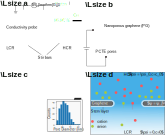
\includegraphics[width=0.95\linewidth]{img/fig1.pdf}
  \caption{\textbf{Experimental setup and nanopore characterization}.
    \textbf{a}. 3D schematic diagram showing the experimental
    setup. Inset: photograph of the PG-PCTE membrane supported by
    Kapton and copper tapes. (Scale bar: 1 cm.) \textbf{b}. 3D schematic
    of the nanoscale cross-sectional structure of the PG-PCTE
    membrane. \textbf{c}. SEM image of the PG-PCTE membrane, showing an
    excellent coverage of graphene over the PCTE substrate, scale bar:
    20 $\mathrm{\mu}$m.  Upper right inset: high-resolution SEM image
    of individual nanopores on PG fabricated by the patterning
    technique. (Scale bar: 500 nm.) Bottom right inset: histogram of the
    pore diameter distribution revealed by the SEM
    image. \textbf{d}. Schematic of the nanoscale ionic transport
    through a gated graphene nanopore.}
  \label{fig:np-1}
\end{figure}

\begin{figure}[H]
  \centering
  % 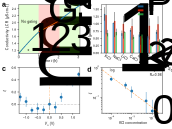
\includegraphics[width=0.95\linewidth]{img/fig2.pdf}
  \caption{ \textbf{The experimental evidence of salt rejection.}
    \textbf{a}. An example of measured conductivity in LCR as a
    function of time. The slope of conductivity-time curve when
    $V_{\mathrm{G}}>0$ is interpolated, is smaller than that without
    gating. \textbf{b}. Molar diffusive flux through bare PCTE (blue
    bars: experimental, $\boldsymbol{J}_{\mathrm{PCTE}}$ Exp.; red
    bars: model values, $\boldsymbol{J}_{\mathrm{PCTE}}$
    ( \autoref{eq:np-j-pcte})) and PG+PCTE
    ($\boldsymbol{J}_{\mathrm{PG0}}$ Exp.; green bars) membranes for
    different salts. \textcolor{blue}{The error bars for
      $\boldsymbol{J}_{\mathrm{PCTE}}$ Exp. were estimated by the
      standard deviation of three consecutive measurements. The error bars
      for $\boldsymbol{J}_{\mathrm{PCTE}}$ ( \autoref{eq:np-j-pcte})
      correspond to the calculated maximum and minimum ion flux values
      using the membrane parameters provided by the vendor. The error
      bars for $\boldsymbol{J}_{\mathrm{PG0}}$ Exp. were estimated by
      the standard deviation of the ion fluxes in the first interval
      during the gating experments.)}  \textbf{c}. Experimentally
    measured salt rejection factor $\xi$ as a function of
    $V_{\mathrm{G}}$ for 0.1 mM KCl solution in HCR, showing an
    asymmetric response, with a higher degree of salt rejection for
    $V_{\mathrm{G}}>0$. \textcolor{blue}{The error bars were estimated
      by the standard deviation for the ion fluxes in the second
      interval during the gating experiments.}
    \textbf{d}. $\xi_{\mathrm{max}}$ as a function of KCl
    concentration, fitted by a power law relation, suggesting the
    effect of Debye length on the observed salt rejection, since
    $\lambda_{\mathrm{D}} \propto c_{0}^{-\frac{1}{2}}$.}
  \label{fig:np-2} 
\end{figure}

\begin{figure}[H]
  \centering
  % 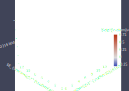
\includegraphics[width=0.95\linewidth]{img/fig3.pdf}
  \caption{\textbf{Interplay between graphene quantum capacitance and
      EDL.} \textbf{a}. Schematic diagram of the electric
    potential at the graphene-electrolyte interface considering the
    quantum capacitance of graphene. The interfacial potential of the
    electrolyte solution, $\psi_{0}$, is smaller than the bias
    $V_{\mathrm{G}}$ applied, as a result of the change of graphene's
    Fermi level $\Delta \phi_{\mathrm{G}}$ and the potential drop in
    the Stern layer $\Delta \psi$. \textbf{b}. Calculated surface
    charge $\sigma_{\mathrm{G}}$ and surface potential
    $\psi_{\mathrm{G}}$ of graphene as a function of $V_{\mathrm{G}}$
    in a 1 mM KCl solution. }
  \label{fig:np-3}
\end{figure}

\begin{figure}[H]
  \centering
  % \includegraphics[width=0.95\linewidth]{img/fig4.pdf}
  \caption{\textbf{Calculations using the proposed self-consistent
      theory}. \textbf{a}. Calculated cross-sectional contour plot of
    electric potential $\psi$ near the center of the graphene
    nanopore at $V_{\mathrm{G}}$ = 0.75 V. \textbf{b}. The
    corresponding electrochemical potential change for cation
    $\Delta \mu_{+}$ (left) and anion $\Delta \mu_{-}$ (right). The
    reference of electrochemical potential is set in the HCR far from
    the graphene layer. The diffusive pathways for both ions are
    indicated by the arrows. \textbf{c}. Calculated z-component of
    diffusive fluxes $\boldsymbol{J}_{z}$ for cation (left) and anion
    (right) through the pore as functions of the relative position
    inside the pore, considering different levels of $V_{\mathrm{G}}$
    applied. \textbf{d}. Calculated z-components of cation, anion, and
    total fluxes through the graphene nanopore as functions of
    $V_{\mathrm{G}}$, showing salt rejection for all fluxes.}
  \label{fig:np-4}
\end{figure}

\begin{figure}[H]
  \centering
  % \includegraphics[width=0.95\linewidth]{img/fig5.pdf}
  \caption{\textbf{The Debye length effect on the degree of salt
      rejection}. \textbf{a}. Calculated contour plot of the surface
    potential of graphene $\psi_{\mathrm{G}}$ as a function of
    $\lambda_{\mathrm{D}}/r_{\mathrm{G}}$ and $V_{\mathrm{G}}$. When
    the Debye length reduces, a higher $V_{\mathrm{G}}$ is required to
    maintain the same surface $\psi_{\mathrm{G}}$
    level. \textbf{b}. Calculated 2D contour plot of theoretically
    predicted $\xi$ as a function of
    $\lambda_{\mathrm{D}}/r_{\mathrm{G}}$ and
    $V_{\mathrm{G}}$. Clearly, a higher degree of salt rejection can
    be achieved by having a higher $V_{\mathrm{G}}$ and
    $\lambda_{\mathrm{D}}/r_{\mathrm{G}}$}
  \label{fig:np-5}
\end{figure}

\begin{figure}[H]
  \centering
  % \includegraphics[width=0.95\linewidth]{img/fig6.pdf}
  \caption{\textbf{Comparison between experimental and theoretical
      salt rejection considering different salt
      species}. \textbf{a}. Experimentally measured $\xi$ as a
    function of $V_{\mathrm{G}}$ for various salts at 0.1 mM. The
    error bar represents the standard error. \textbf{b}. Theoretically
    calculated $\xi-V_{\mathrm{G}}$ relations for the salt species
    considered here. \textbf{c}. Comparison between the experimental
    and calculated $\xi_{\mathrm{max}}$ values for different salt
    species, decreasing with the salt
    valence. \textbf{d}. $\xi_{\mathrm{max}}$ as a function of
    $\lambda_{\mathrm{D}}$ for the experimental (circle) and model
    (diamonds) values, showing a linear correlation.}
  \label{fig:np-6}
\end{figure}







%%% Local Variables:
%%% mode: latex
%%% TeX-master: "../thesis"
%%% End:
